\section{Second Models Comparison}
\label{part5}

\subsection{Testing protocol definition}


Each comparison is presented using as element of comparison the metrics \textit{Coverage} and \textit{bandwidth}, as defined in section \ref{other_metrics}
The models uses the custom loss as defined in section \ref{loss} if this loss can be implemented.

The plot results are all presented with the same values of quantiles, the quantile $quantile(0.99)$ and the respective $quantile(0.01)$ but also the $quantile(0.9)$, $quantile(0.1)$ and the median.
Before the comparison between different models, we need to compare the impact of the values of the different hyperparameters of the problem.
The hyperparameters of the problem are :
\begin{itemize}
\item The alpha value, as defined in section \ref{custom_loss}
    \item The learning rate of the model training
    \item The number of epochs of the training
    \item The output distribution, defined in section \ref{distribution}
    \item The individual hyperparameters of the different models
\end{itemize}
Each comparison section is interested in one particular hyperparameter of the problem.
In general the other hyperparameters takes default values, as given by GluonTS.

\subsection{Global Hyperparameters comparison}

\subsubsection{Alpha} \label{comp2_alpha}

\begin{figure}[!h]
    \centering
    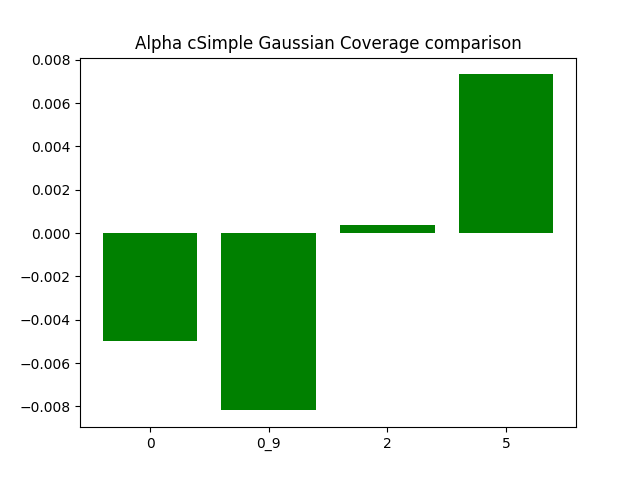
\includegraphics[width=300px]{plots/hist/a/alpha/cSimple/Gaussian/Coverage.png}
    %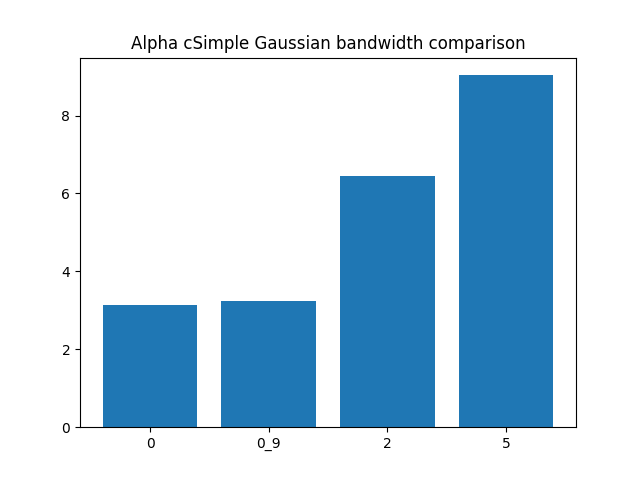
\includegraphics[width=200px]{plots/hist/a/alpha/cSimple/Gaussian/bandwidth.png}
    %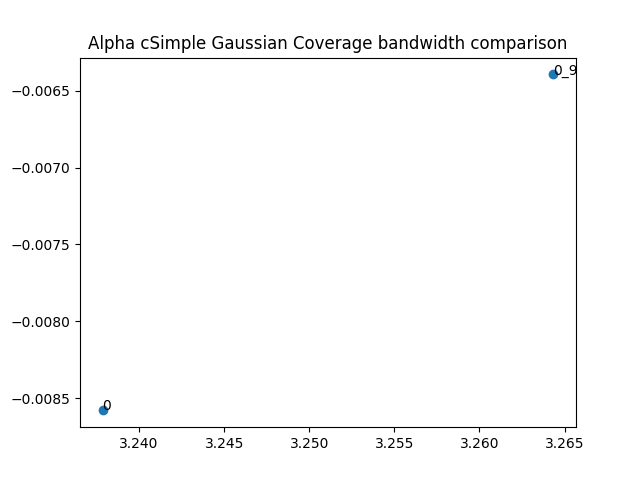
\includegraphics[width=300px]{plots/scatter/a/alpha/cSimple/Gaussian/Coverage_bandwidth.png}
    \caption{Comparison of different $\alpha$ values (Model: Simple (Default parameter values), Epochs = 100, Distribution = Gaussian, Config A)}
    \label{fig:comp2_alpha}
\end{figure}

The value of $\alpha$, defined in section \ref{loss} influence the model behaviour.
Bandwidth value decrease with alpha, as Coverage increase with alpha, which tends to show the efficiency of the custom loss.



\subsubsection{Time series size} \label{comp2_datasize}

\begin{figure}[H]
    \centering
    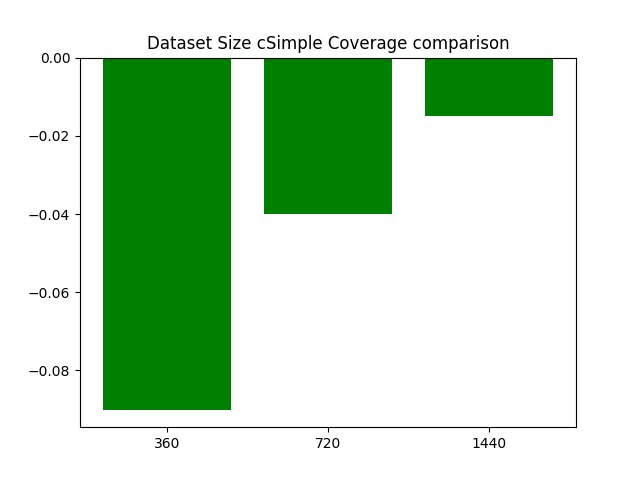
\includegraphics[width=300px]{plots/hist/a/datasize/cSimple/Coverage.png}
    %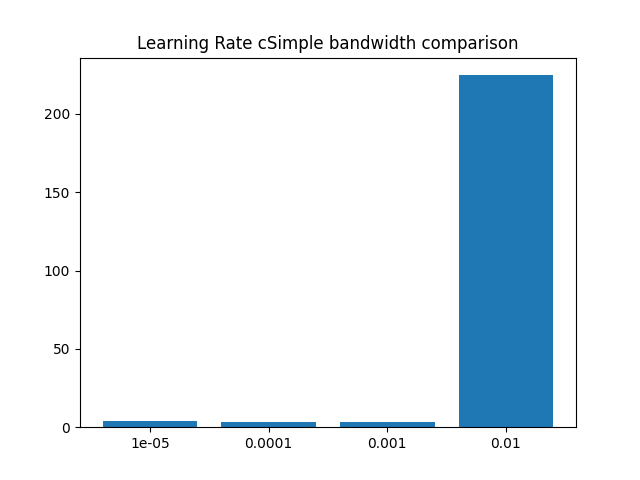
\includegraphics[width=200px]{plots/hist/a/lr/cSimple/bandwidth.png}
    %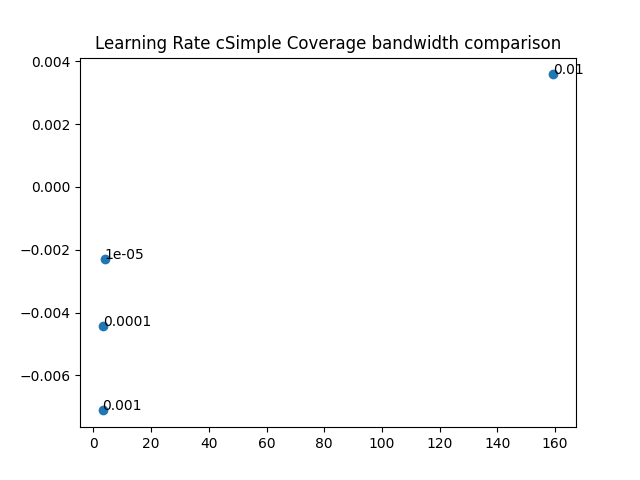
\includegraphics[width=300px]{plots/scatter/a/lr/cSimple/Coverage_bandwidth.png}
    \caption{Comparison of different time series size (Model: Simple (Default parameter values), Epochs = 100, $\alpha$ = 0.9, Distribution = Gaussian, Config A)}
    \label{fig:comp2_datasize}
\end{figure}


\subsubsection{Learning rate} \label{comp2_lr}

\begin{figure}[H]
    \centering
    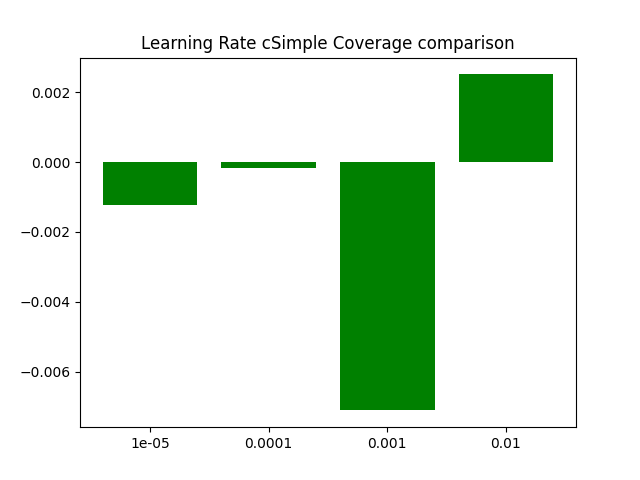
\includegraphics[width=300px]{plots/hist/a/lr/cSimple/Coverage.png}
    %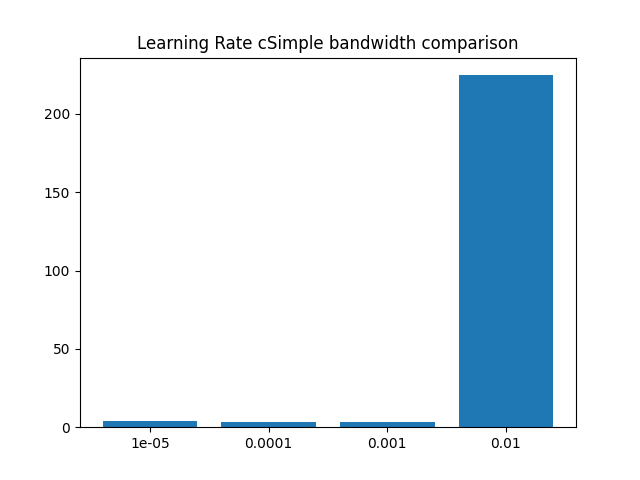
\includegraphics[width=200px]{plots/hist/a/lr/cSimple/bandwidth.png}
    %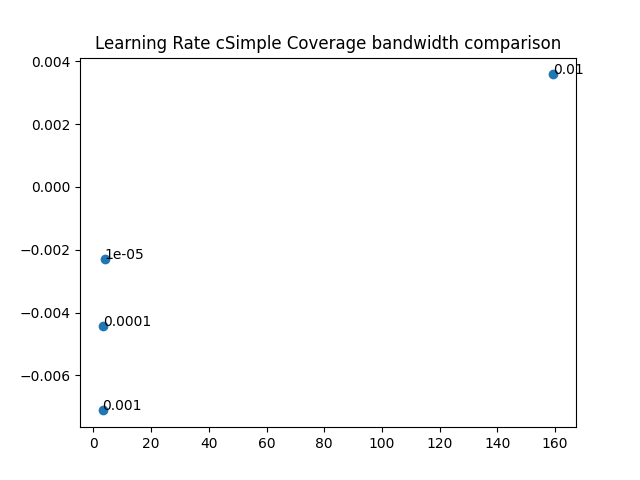
\includegraphics[width=300px]{plots/scatter/a/lr/cSimple/Coverage_bandwidth.png}
    \caption{Comparison of different learning rate (Model: Simple (Default parameter values), Epochs = 100, $\alpha$ = 0.9, Distribution = Gaussian, Config A)}
    \label{fig:comp2_lr}
\end{figure}

The default learning rate in GluonTs for all deep learning models is $1^{-3}$
Learning rate as a great impact on the results.

\subsubsection{Epochs} \label{comp2_epochs}

\begin{figure}[H]
    \centering
    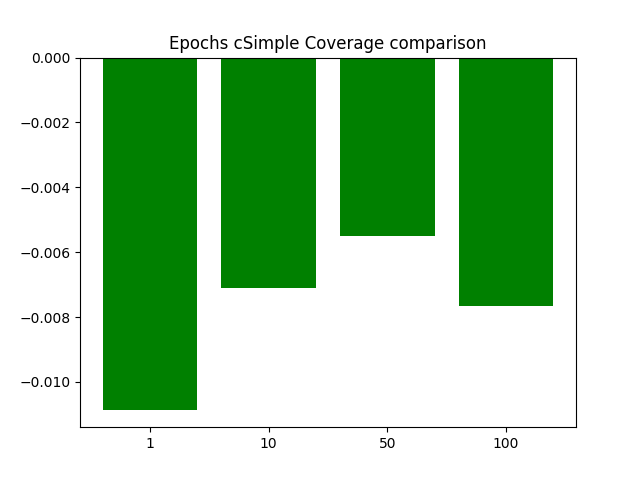
\includegraphics[width=300px]{plots/hist/a/epochs/cSimple/Coverage.png}
    %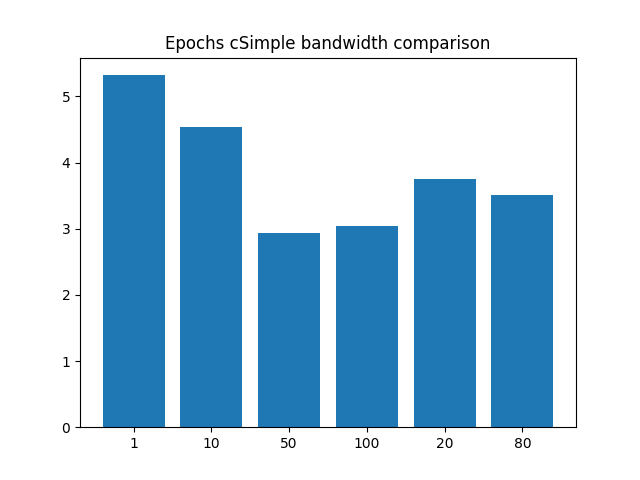
\includegraphics[width=200px]{plots/hist/a/epochs/cSimple/bandwidth.png}
    %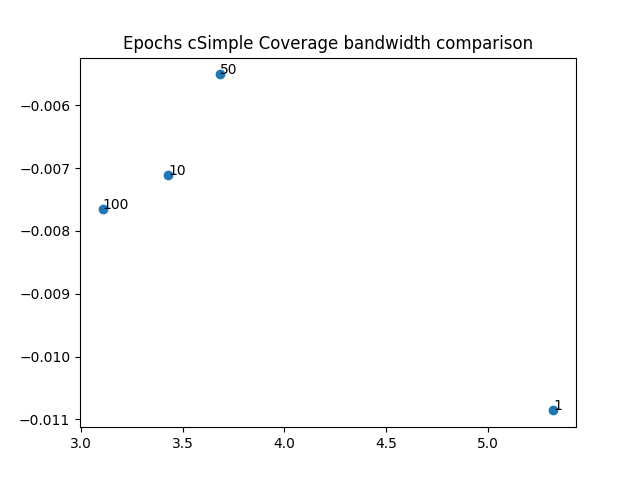
\includegraphics[width=300px]{plots/scatter/a/epochs/cSimple/Coverage_bandwidth.png}
    \caption{Comparison of different epochs number (Model: Simple (Default parameter values), $\alpha$ = 0.9, Distribution = Gaussian, Config A)}
    \label{fig:comp2_epochs}
\end{figure}

All the deep learning models implemented must be trained a certain number of epochs. The default number 
is 100 epochs. This value is a good choice (better bandwidth of the comparison), as are values slightly  inferior (which have better Coverage). 

\newpage

\subsubsection{Output Distribution} \label{comp2_outdistrib}

\begin{figure}[H]
    \centering
    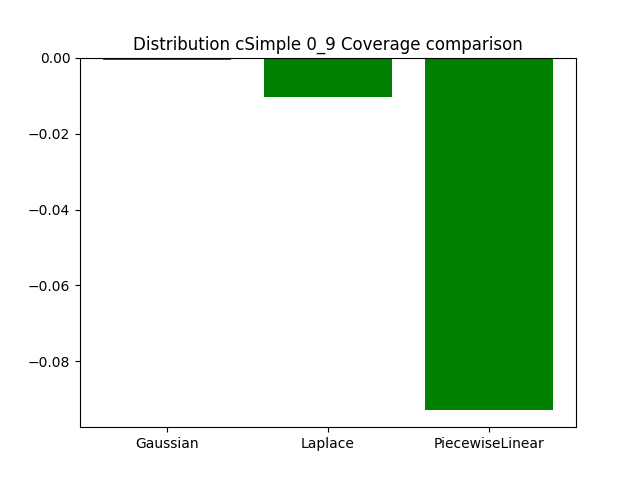
\includegraphics[width=300px]{plots/hist/a/distribution/cSimple/0_9/Coverage.png}
    %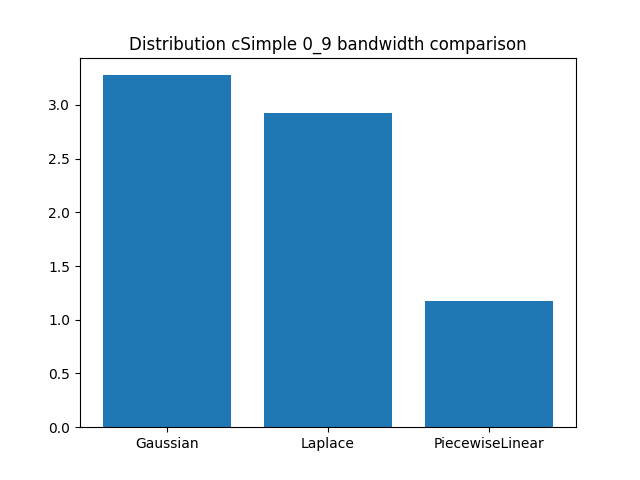
\includegraphics[width=200px]{plots/hist/a/distribution/cSimple/0_9/bandwidth.png}
    %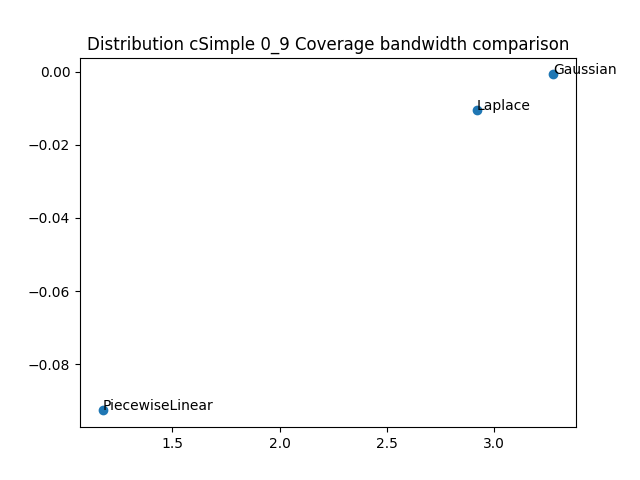
\includegraphics[width=300px]{plots/scatter/a/distribution/cSimple/0_9/Coverage_bandwidth.png}
    \caption{Comparison of different output distribution (Model: Simple (Default parameter values), Epochs = 100, $\alpha$ = 0.9,  Config A)}
    \label{fig:comp2_outdistrib}
\end{figure}

% \textit{PiecewiseLinear} distribution gives very thin distribution but clearly underestimate the risk, and would be not chosen in consequence. Laplace gives slightly better results than Gaussian if we consider Coverage and bandwith as the same level of importance. 


\subsection{Different models parameters comparison and results} \label{comp2_model_param}

The different models are described in the \ref{diff_models} section

\subsubsection{Simple} \label{comp2_simple}

\begin{figure}[H]
    \centering
    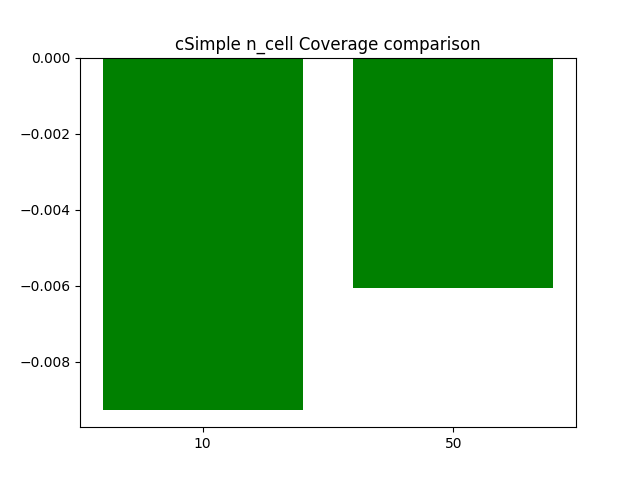
\includegraphics[width=300px]{plots/hist/a/cSimple/n_cell/Coverage.png}
    %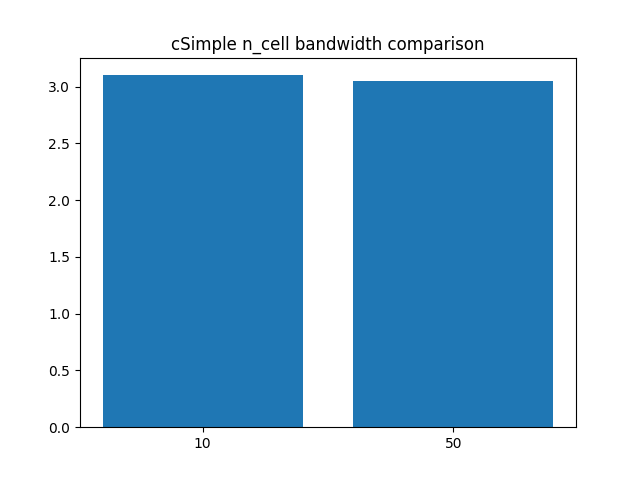
\includegraphics[width=200px]{plots/hist/a/cSimple/n_cell/bandwidth.png}
    %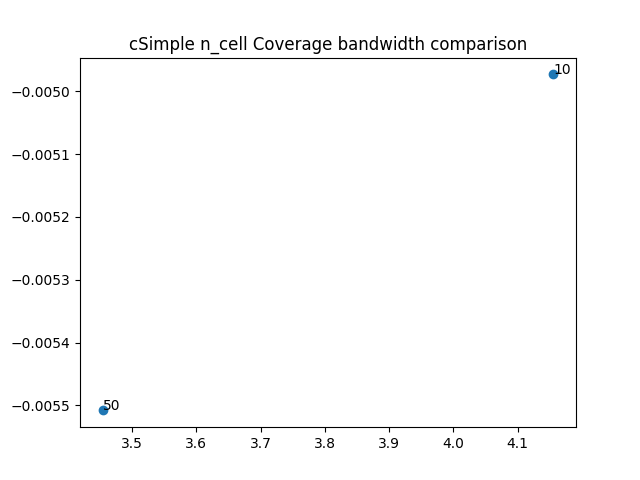
\includegraphics[width=300px]{plots/scatter/a/cSimple/n_cell/Coverage_bandwidth.png}
    \caption{Comparison of different $n\_cell$ values for Simple model (Epochs = 100, Distribution = Gaussian, $\alpha = 0.9$, Config A)}
    \label{fig:comp2_simple}
\end{figure}



\subsubsection{Simple Feed Fordward} \label{comp2_feedfordward}

\begin{figure}[H]
    \centering
    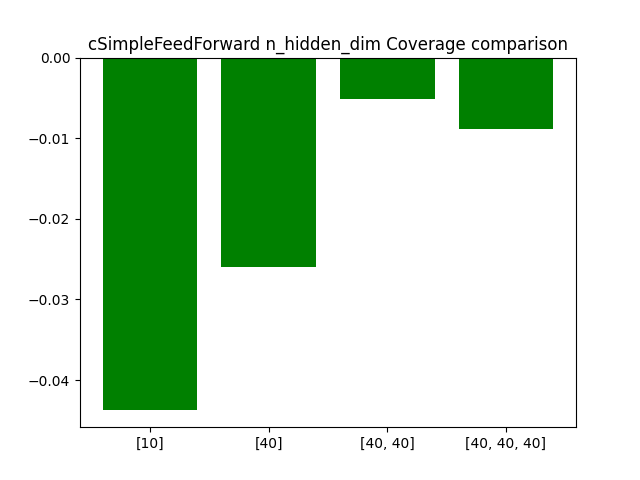
\includegraphics[width=300px]{plots/hist/a/cSimpleFeedForward/n_hidden_dim/Coverage.png}
    %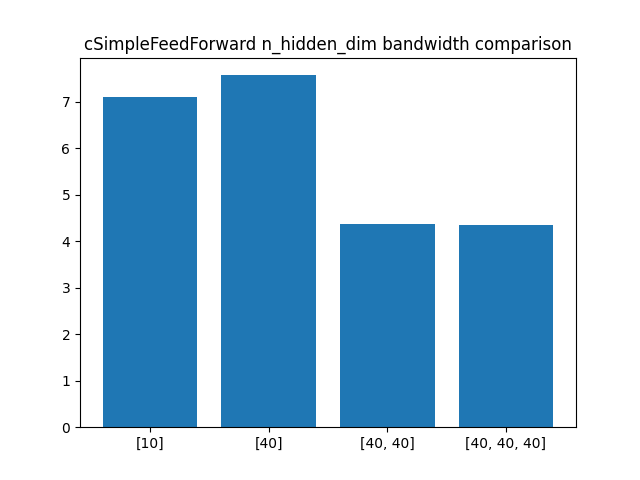
\includegraphics[width=200px]{plots/hist/a/cSimpleFeedForward/n_hidden_dim/bandwidth.png}
    %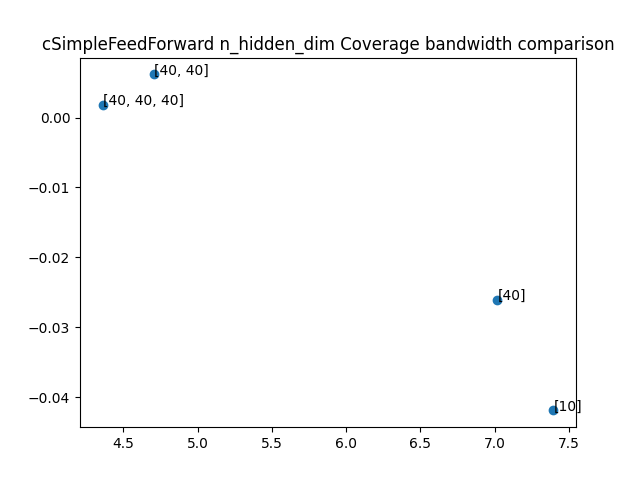
\includegraphics[width=300px]{plots/scatter/a/cSimpleFeedForward/n_hidden_dim/Coverage_bandwidth.png}
    \caption{Comparison of different $n\_hidden\_dim$ values for Simple FeedForward model (Epochs = 100, Distribution = Gaussian, $\alpha = 0.9$, Config A)}
    \label{fig:comp2_feedfordward}
\end{figure}



\subsubsection{Canonical RNN} \label{comp2_canonicalrnn}

\begin{figure}[H]
    \centering
    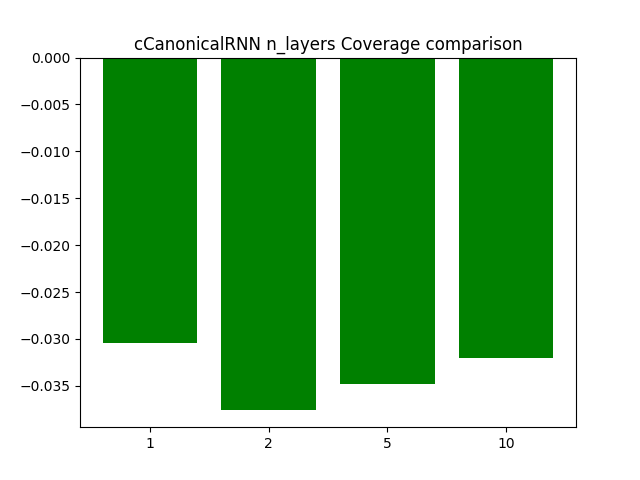
\includegraphics[width=300px]{plots/hist/a/cCanonicalRNN/n_layers/Coverage.png}
    %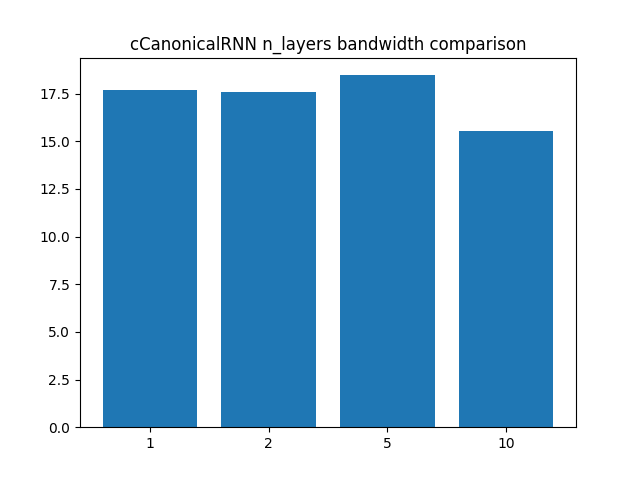
\includegraphics[width=200px]{plots/hist/a/cCanonicalRNN/n_layers/bandwidth.png}
    %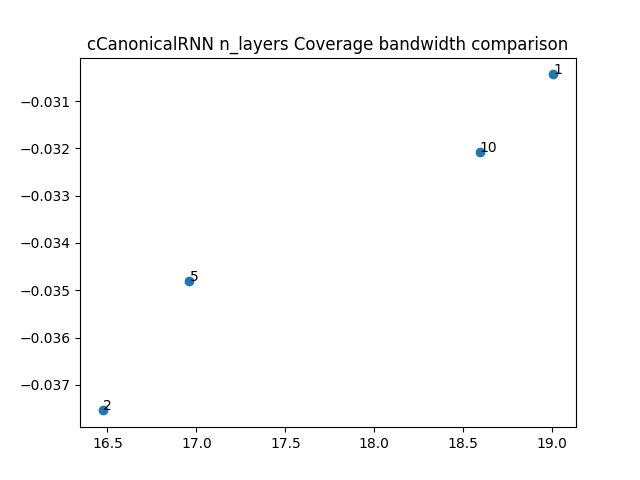
\includegraphics[width=300px]{plots/scatter/a/cCanonicalRNN/n_layers/Coverage_bandwidth.png}
    \caption{Comparison of different $n\_layers$ values for Canonical RNN model (Epochs = 100, Distribution = Gaussian, $\alpha = 0.9$, Config A)}
    \label{fig:comp2_canonicalrnn}
\end{figure}



\subsubsection{Deep AR} \label{comp2_deepar}

\begin{figure}[H]
    \centering
    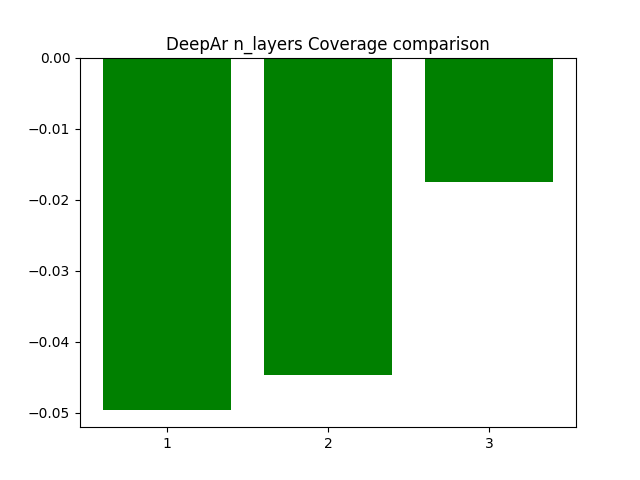
\includegraphics[width=300px]{plots/hist/a/DeepAr/n_layers/Coverage.png}
    %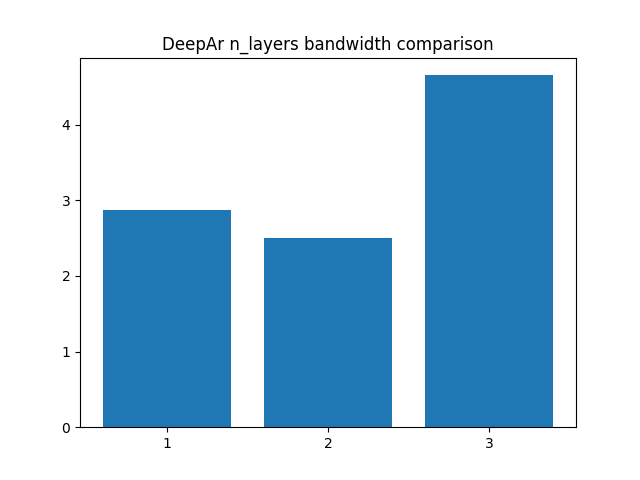
\includegraphics[width=200px]{plots/hist/a/DeepAr/n_layers/bandwidth.png}
    %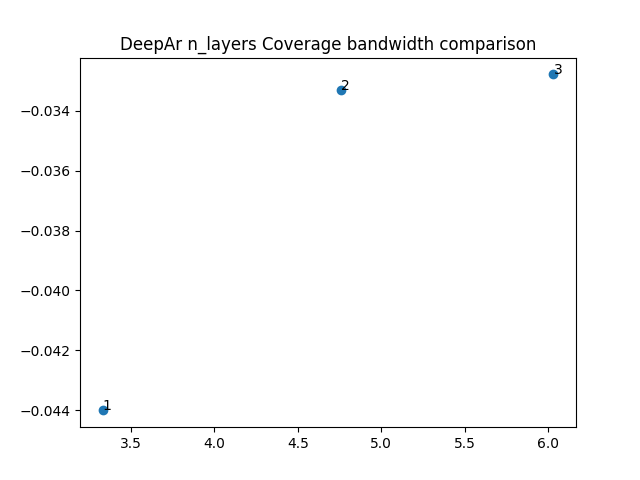
\includegraphics[width=300px]{plots/scatter/a/DeepAr/n_layers/Coverage_bandwidth.png}
    \caption{Comparison of different $n\_layers$ values for Deep AR model (Epochs = 100, Distribution = Gaussian, Config A)}
    \label{fig:comp2_deepar_n_layers}
\end{figure}

\begin{figure}[H]
    \centering
    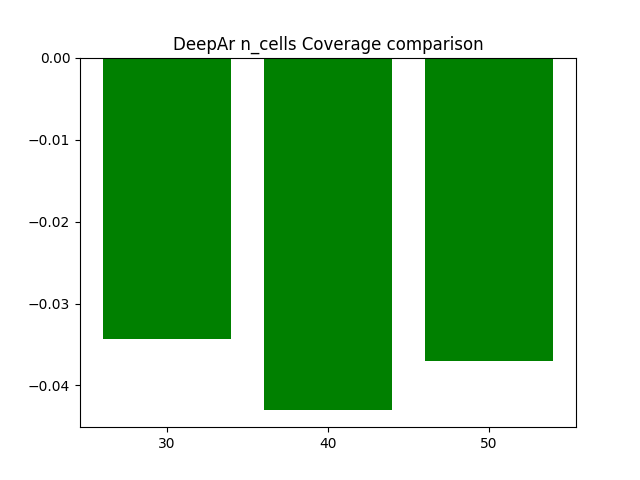
\includegraphics[width=300px]{plots/hist/a/DeepAr/n_cells/Coverage.png}
    %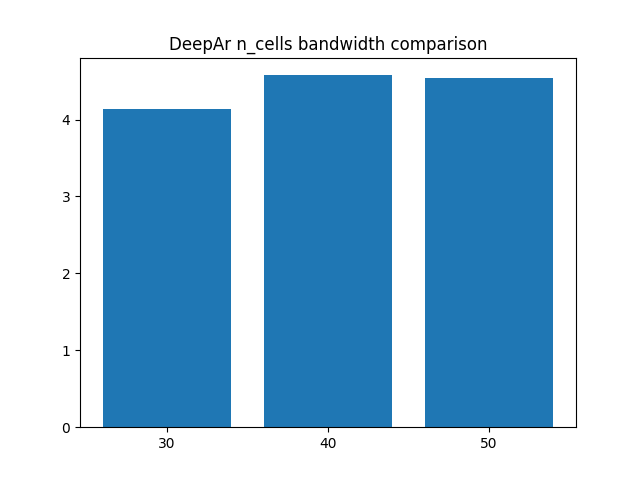
\includegraphics[width=200px]{plots/hist/a/DeepAr/n_cells/bandwidth.png}
    %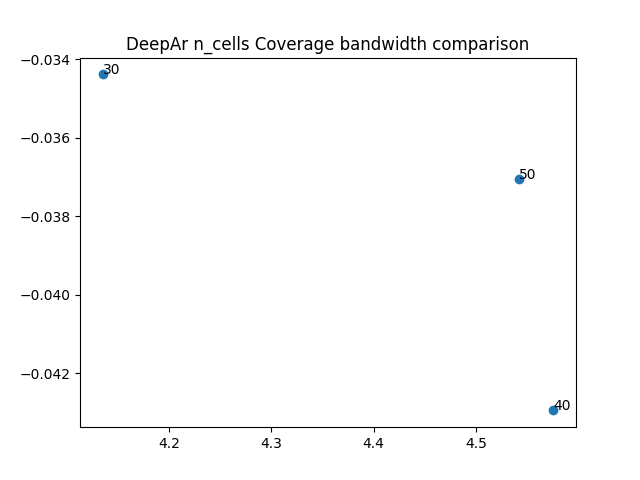
\includegraphics[width=300px]{plots/scatter/a/DeepAr/n_cells/Coverage_bandwidth.png}
    \caption{Comparison of different $n\_cells$ values for Deep AR model (Epochs = 100, Distribution = Gaussian, Config A)}
    \label{fig:comp2_deepar_n_cells}
\end{figure}

\subsubsection{Deep Factor} \label{comp2_deepfactor}

\begin{figure}[H]
    \centering
    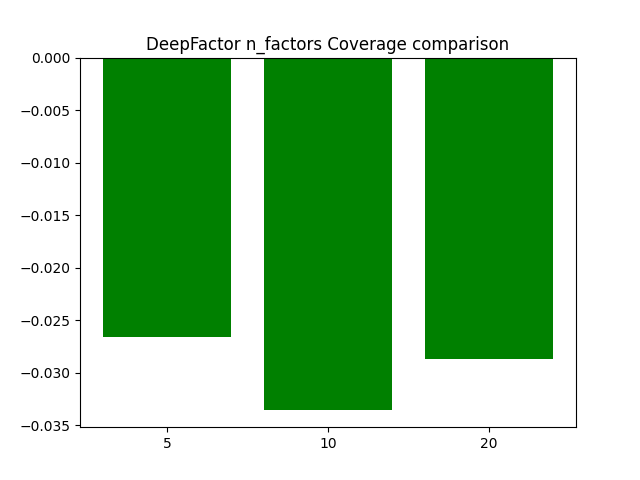
\includegraphics[width=300px]{plots/hist/a/DeepFactor/n_factors/Coverage.png}
    %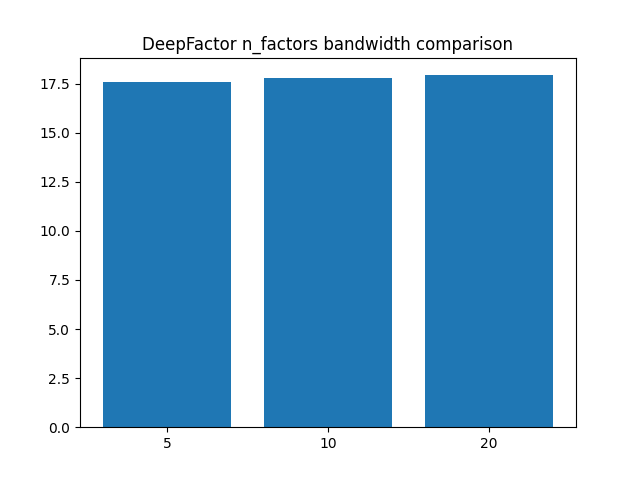
\includegraphics[width=200px]{plots/hist/a/DeepFactor/n_factors/bandwidth.png}
    %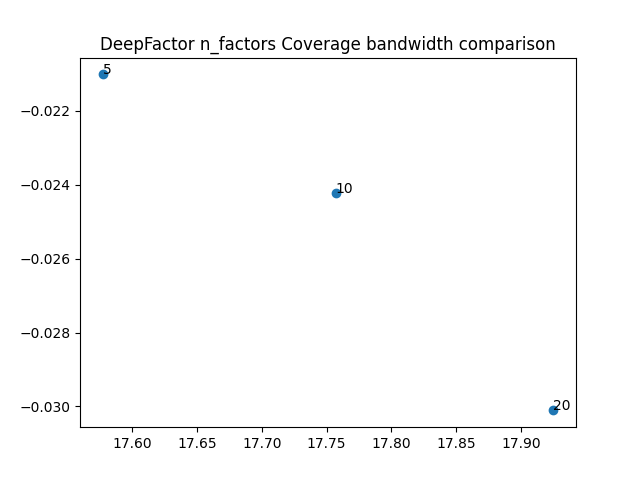
\includegraphics[width=300px]{plots/scatter/a/DeepFactor/n_factors/Coverage_bandwidth.png}
    \caption{Comparison of different $n\_factors$ values for Deep Factors model (Epochs = 100, Distribution = Gaussian, $\alpha = 0.9$, Config A)}
    \label{fig:comp2_deepfactor_n_factors}
\end{figure}

\begin{figure}[H]
    \centering
    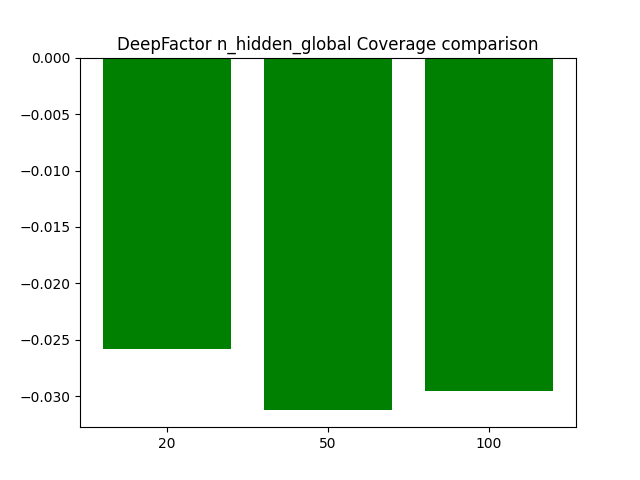
\includegraphics[width=300px]{plots/hist/a/DeepFactor/n_hidden_global/Coverage.png}
    %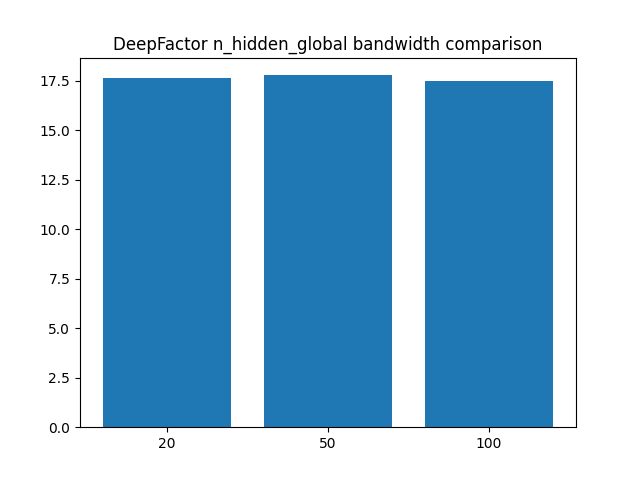
\includegraphics[width=200px]{plots/hist/a/DeepFactor/n_hidden_global/bandwidth.png}
    %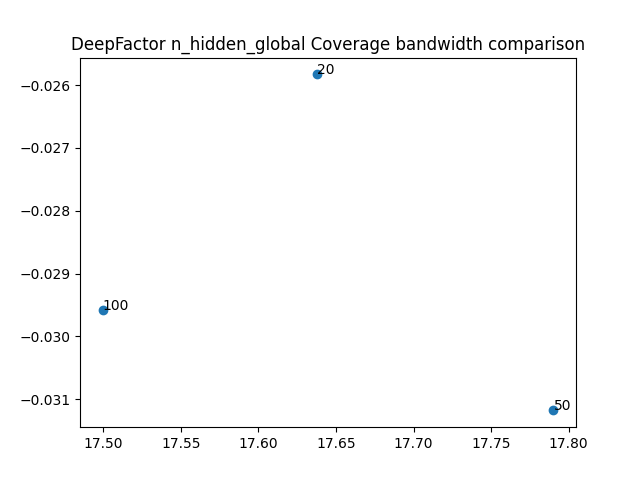
\includegraphics[width=300px]{plots/scatter/a/DeepFactor/n_hidden_global/Coverage_bandwidth.png}
    \caption{Comparison of different $n\_hidden\_global$ values for Deep Factors model (Epochs = 100, Distribution = Gaussian, $\alpha = 0.9$, Config A)}
    \label{fig:comp2_deepfactor_n_hidden_globals}
\end{figure}

\begin{figure}[H]
    \centering
    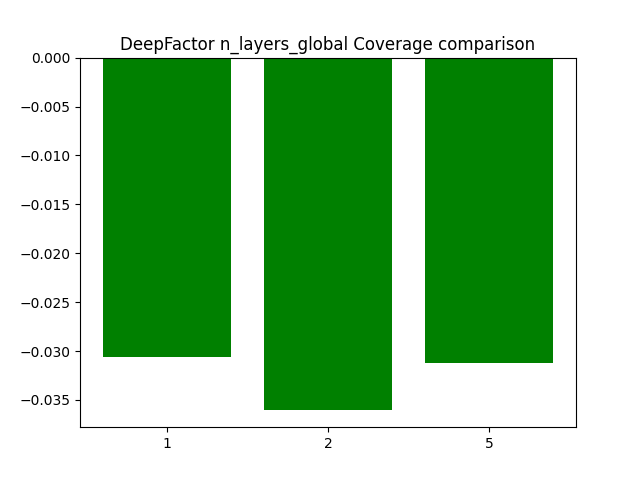
\includegraphics[width=300px]{plots/hist/a/DeepFactor/n_layers_global/Coverage.png}
    %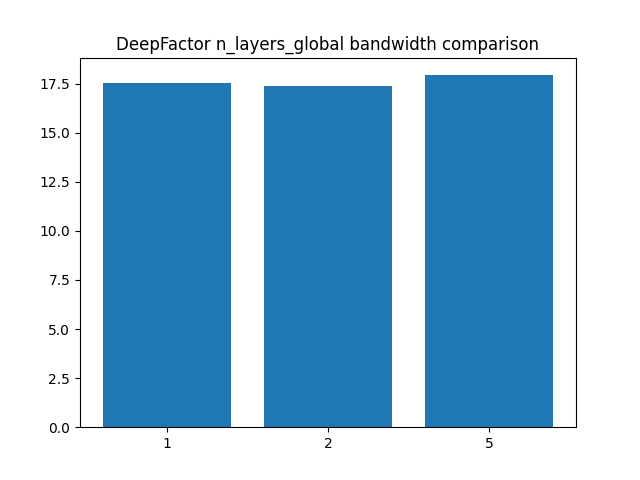
\includegraphics[width=200px]{plots/hist/a/DeepFactor/n_layers_global/bandwidth.png}
    %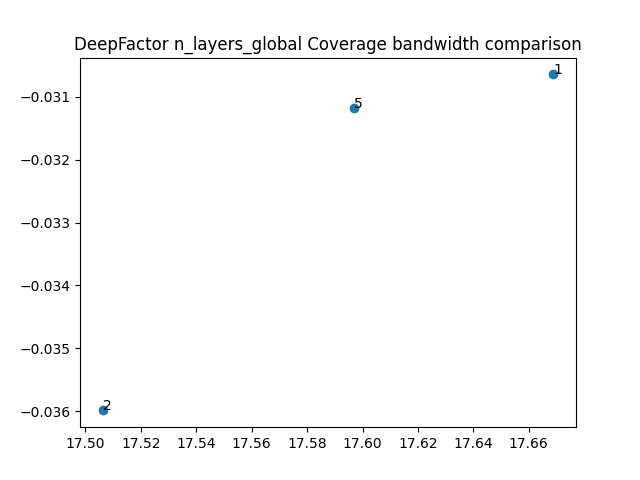
\includegraphics[width=300px]{plots/scatter/a/DeepFactor/n_layers_global/Coverage_bandwidth.png}
    \caption{Comparison of different $n\_layers\_global$ values for Deep Factors model (Epochs = 100, Distribution = Gaussian, $\alpha = 0.9$, Config A)}
    \label{fig:comp2_deepfactor_n_layers_global}
\end{figure}

Contrary to another model, different hyperparameters of Deep Factors had a relatively low impact on the quality of the model.

\subsubsection{MQCNN} \label{comp2_mqcnn}

\begin{figure}[H]
    \centering
    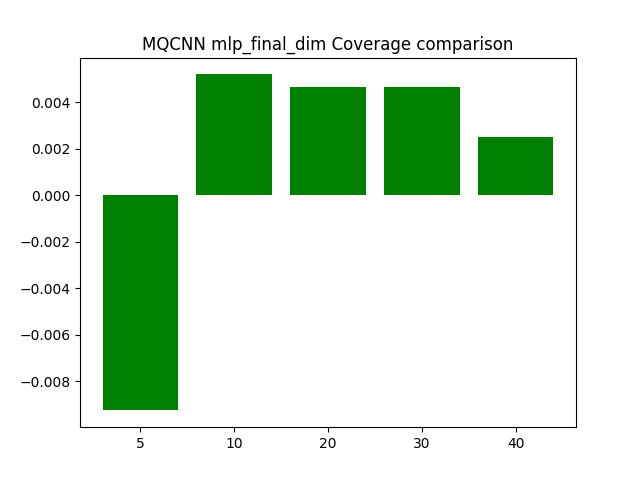
\includegraphics[width=300px]{plots/hist/a/MQCNN/mlp_final_dim/Coverage.png}
    %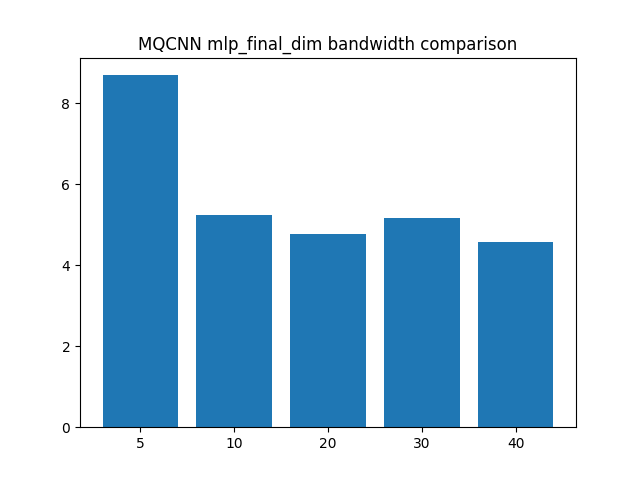
\includegraphics[width=200px]{plots/hist/a/MQCNN/mlp_final_dim/bandwidth.png}
    %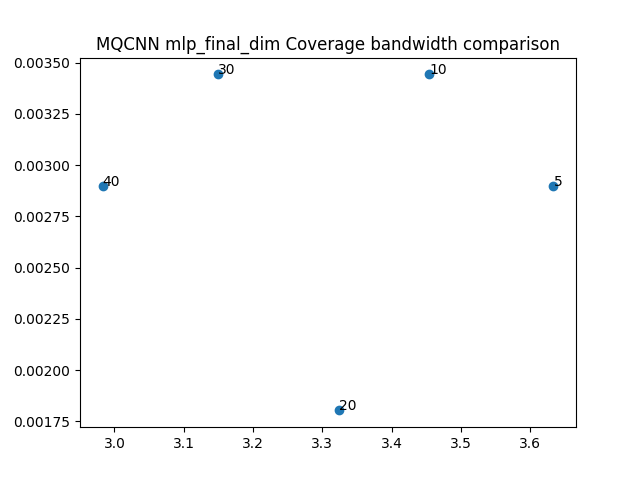
\includegraphics[width=300px]{plots/scatter/a/MQCNN/mlp_final_dim/Coverage_bandwidth.png}
    \caption{Comparison of different $mlp\_final\_dim$ values for MQCNN model (Epochs = 100, Distribution = Gaussian, Config A)}
    \label{fig:comp2_mqcnn}
\end{figure}

\subsubsection{MQRNN} \label{comp2_mqrnn}

\begin{figure}[H]
    \centering
    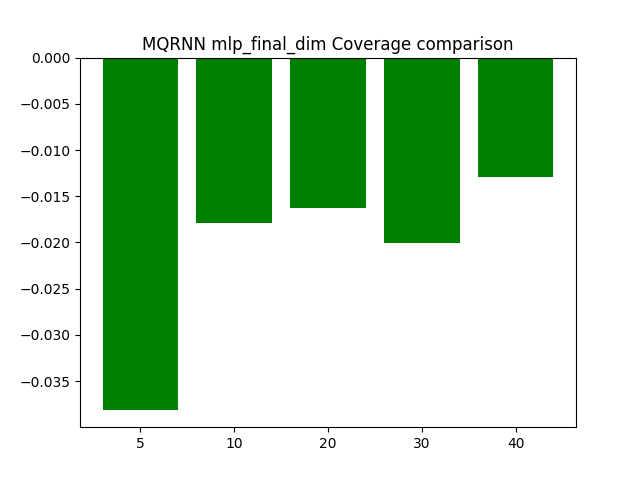
\includegraphics[width=300px]{plots/hist/a/MQRNN/mlp_final_dim/Coverage.png}
    %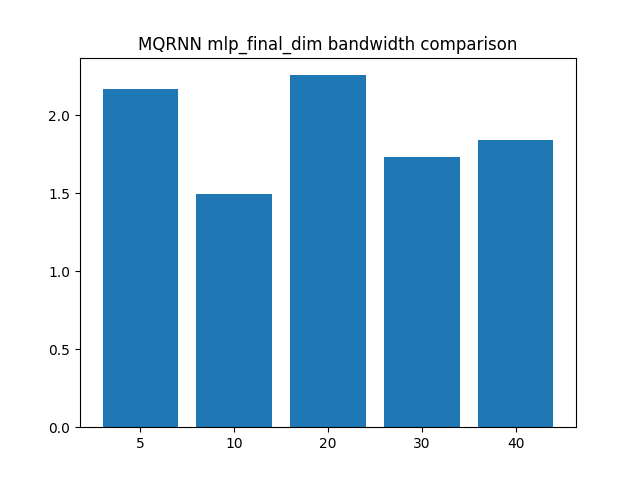
\includegraphics[width=200px]{plots/hist/a/MQRNN/mlp_final_dim/bandwidth.png}
    %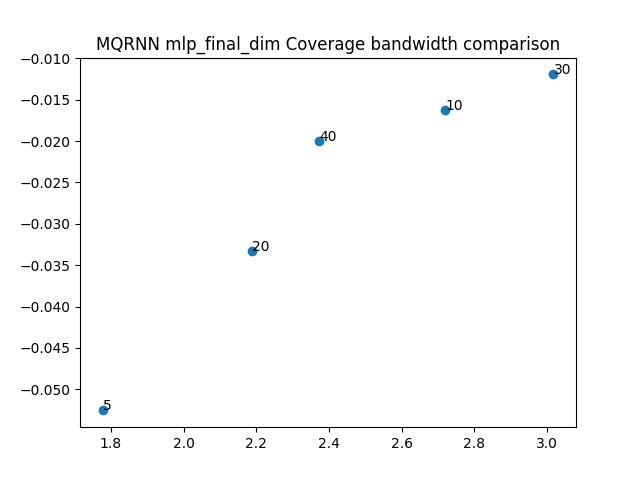
\includegraphics[width=300px]{plots/scatter/a/MQRNN/mlp_final_dim/Coverage_bandwidth.png}
    \caption{Comparison of different $mlp\_final\_dim$ values for MQRNN model (Epochs = 100, Distribution = Gaussian, Config A)}
    \label{fig:comp2_mqrnn}
\end{figure}


\subsection{Global comparison}

\begin{figure}[H]
    \centering
    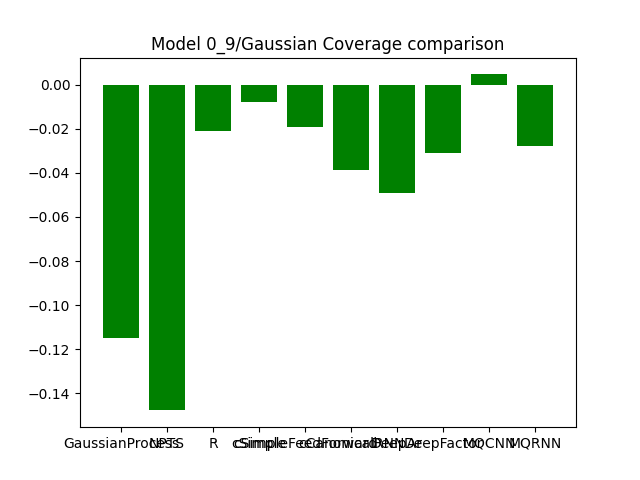
\includegraphics[width=200px]{plots/hist/a/model/0_9/Gaussian/Coverage.png}
    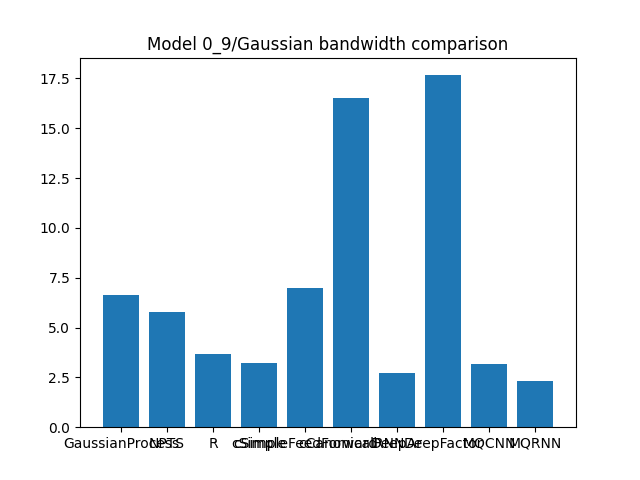
\includegraphics[width=200px]{plots/hist/a/model/0_9/Gaussian/bandwidth.png}
    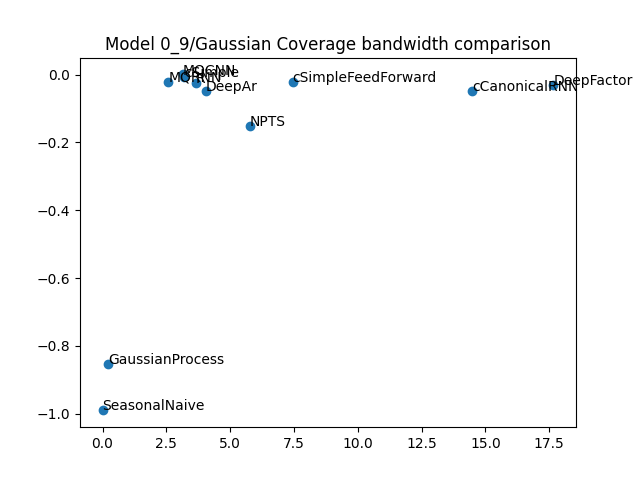
\includegraphics[width=300px]{plots/scatter/a/model/0_9/Gaussian/Coverage_bandwidth.png}
    \caption{Comparison of different models (Epochs = 100, Distribution = Gaussian, Config A)}
    \label{fig:comp2_mqcnn}
\end{figure}

Now that all the hyperparameters has been studied, all the tuned models can be compared to infer a hierarchy of the model which forecast the different configuration the better. This will leave us to the question at the base of this work.

The first observation is that DeepFactor and CanonicalRNN underperform in term of bandwidth compared to the others.
The second is that Gaussian Process and NPTS underperform in terms of Coverage compared to the others.
It leaves us 6 models.
The better model in terms of bandwidth, with an acceptable Coverage if we consider that this window of value is acceptable is MQRNN.
The better model in terms of Coverage is MQCNN. It Coverage is not only higher than others, but positive. 
Simple model gives impressive results considering the simplicity of it implementation.
The ETS model gives good results as the only not deep learning model.